\documentclass[utf8x, 12pt]{G7-32} 


% --------- -------- SETTINGS --------- --------

% --------- Настройки стиля ГОСТ 7-32 --------

% Гипертекстовое оглавление в PDF
\usepackage[
bookmarks=true, colorlinks=true, unicode=true,
urlcolor=black,linkcolor=black, anchorcolor=black,
citecolor=black, menucolor=black, filecolor=black,
]{hyperref}

\usepackage{graphicx}   % Пакет для включения рисунков
\DeclareGraphicsExtensions{.jpg,.pdf,.png}
\geometry{right=20mm}
\geometry{left=30mm}
\usepackage{enumerate}
\setcounter{tocdepth}{3} % Подробность оглавления


% --------- other settings --------
\usepackage{MnSymbol}
%\usepackage{simpsons}
% --------- -------- SETTINGS --------- --------



\begin{document}

\frontmatter 

% --------- -------- TITLE --------- --------

\begin{center} 

\large САНКТ-ПЕТЕРБУРГСИЙ ГОСУДАРСТВЕННЫЙ ПОЛИТЕХНИЧЕСКИЙ УНИВЕРСИТЕТ

\large Кафедра Компьютерных Систем и Программных Технологий \\[5.5cm] 

\huge ОТЧЕТ \\[0.6cm] % название работы, затем отступ 0,6см
\large по лабораторной работе №4\\
\large Тема: <<Утилита для исследования сети и сканер портов Nmap>>\\
\large Дисциплина: <<Методы и средства защиты информации>>\\[3.7cm]

\end{center} 

\begin{flushright}
Выполнил: студент гр. 53501/2 \\
Пономарев М.A. \\[1.2cm]


Преподаватель \\
Вылегжанина К.Д.
\end{flushright}


\vfill 

\begin{center} 
\large Санкт-Петербург \\
2015
\end{center} 

\thispagestyle{empty}


% --------- -------- TITLE --------- --------

\thispagestyle{empty}
\setcounter{page}{0}
\tableofcontents
\clearpage
\mainmatter


\chapter{Задание}

\begin{enumerate}
	\item Проверить поиск активных хостов
	\item Определить открытые порты
	\item Определить версии сервисов
	\item Изучить файлы nmap-services, nmap-os-db, nmap-service-probes
	\item Добавить новую сигнатуру службы в файл nmap-service-probes (для этого создать минимальный tcp server, добиться, чтобы при сканировании nmap указывал для него название и версию)
	\item Сохранить вывод утилиты в формате xml
	\item Исследовать различные этапы и режимы работы nmap с использованием утилиты Wireshark
\end{enumerate}


\chapter{Выполнение}


\section{Проверить поиск активных хостов}



\section{Определить открытые порты}
\section{Определить версии сервисов}
\section{Изучить файлы nmap-services, nmap-os-db, nmap-service-probes}
\section{Добавить новую сигнатуру службы в файл nmap-service-probes}
\section{Сохранить вывод утилиты в формате xml}
\section{Исследовать различные этапы и режимы работы nmap с использованием утилиты Wireshark}


\begin{figure}[hhh!]
	\begin{center}
		%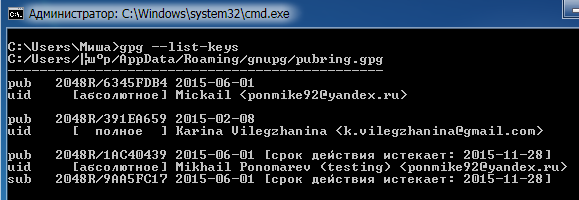
\includegraphics[width=12cm]{img/8_2}
	\end{center}
\end{figure}	


\end{document}
